\section{The tie and its resolution}\label{sec:simplex-thresholds}

In this section the start is uniform. We prove the tie of
Section~\ref{sec:question} and break it (Subsection~\ref{sec:tie}), write the
constants as Gaussian volumes and spanning-tree sums
(Subsection~\ref{sec:gaussian-volumes}), and find the global mode
(Subsection~\ref{sec:global-mode}). The constants $a_k$, $D_k$ and $\Psi_N$ are
those of~\eqref{eq:intro-ak}. Let $n$ be a balanced vector with $k$ positive
coordinates and total $N$. By Proposition~\ref{prop:dpmf}(b),
$C_{N,k}/V_N=S_n(u)$, and as a function of $u$ this ratio does not depend
on $d$.

\subsection{Every face ties at first order}\label{sec:tie}

\begin{theorem}[every face ties at first order]\label{thm:simplex-window}
Fix $d\ge2$ and $0<c<C$.
\begin{enumerate}[(i)]
\item For large $N$, uniformly for $cL\le T\le CL$ and $2\le k\le d$,
\[
\log\frac{C_{N,k}}{V_N}=(k-1)\bigl[\Psi_N(T)-a_k\bigr]-\frac{k-1}{8T}
+O\Bigl(\frac1{T^2}+\frac{T^2}N\Bigr).
\]
\item Put $T=\tau L$. Uniformly for $c\le\tau\le C$ and $1\le k\le d$, a face
$F$ with $k$ states has
\[
\log C_{N,k}=-L\bigl[\tau\lambda_F+k-1\bigr]+O(\log L),\qquad\lambda_F=d-k .
\]
At $\tau=1$ the right side is $-(d-1)L+O(\log L)$ for every $k$.
\item Put $T=L-\frac12\log L+t$. Uniformly for $t$ in a compact interval, for
each $2\le k\le d$,
\begin{equation}\label{eq:simplex-window}
\frac{C_{N,k}}{V_N}\longrightarrow e^{(k-1)(t-a_k)} .
\end{equation}
\item $a_2>a_3>\cdots$.
\end{enumerate}
\end{theorem}

In words, the central bin of every face reaches the vertices when $\Psi_N(T)$
is of order $1$, that is, when $T=L-\frac12\log L+O(1)$. Part (ii) is the
first-order statement: on the scale $L$ all faces have the same exponent at
$\tau=1$. Part (iii) zooms into the window where the tie lives. There each ratio
has a limit, and the faces differ only through the constants $a_k$. Paper~C
describes such tie windows in general, and Remark~\ref{rem:sticky} explains why
among symmetric kernels only the uniform one ties on every face.

\begin{theorem}[face-center crossings]\label{thm:simplex-crossing}
For every $2\le k\le d$ and $N\ge k$ there is exactly one $p=p_{N,k}\in(0,1)$
with $C_{N,k}(p)=V_N(p)$. The balanced bin is more likely than a vertex below
$p_{N,k}$ and less likely above it. The crossing $p_{N,k}$ is strictly
increasing in $N$,
\[
p_{k,k}=\frac1{1+(d-1)(k!)^{-1/(k-1)}},
\]
and every crossing has $u\le(k!)^{-1/(k-1)}<1$, so $p_{N,k}>1/d$. For fixed $k$
the value $z_{N,k}=N(1-p_{N,k})/(d-1)$ of $T$ at the crossing satisfies
\[
z_{N,k}+\frac12\log z_{N,k}=L+a_k+\frac1{8z_{N,k}}+O(L^{-2}),
\]
and
\begin{equation}\label{eq:simplex-root-expansion}
z_{N,k}=L-\frac12\log L+a_k
+\frac{\frac14\log L-\frac12a_k+\frac18}{L}
+O\Bigl(\frac{(\log L)^2}{L^2}\Bigr).
\end{equation}
\end{theorem}

In words, each face center crosses the vertices exactly once, the crossing
moves towards $p=1$ as $N$ grows, and the crossing equation is the same for
every face except for the constant $a_k$. For $d=2$, $z_{N,2}=N(1-p_N)$ is the
crossing $z_N$ of~\cite{paperA}, and $a_2=\frac12\log(\pi/8)$ is its constant
$c_0$. The proofs here do not use the binary case.
Figure~\ref{fig:simplex} shows the full-center crossing on the triangle at
$N=24$.

\begin{figure}[t]
\centering
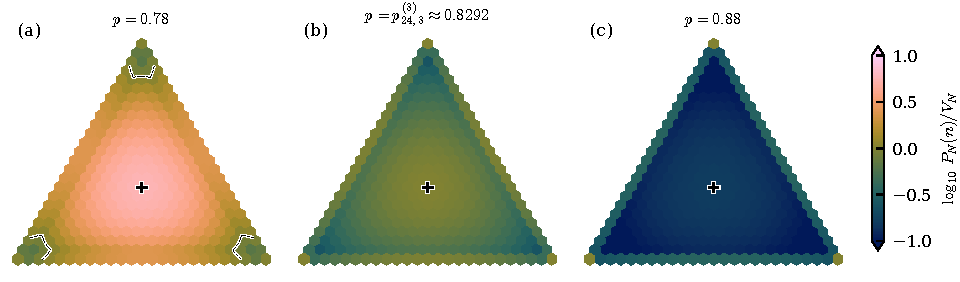
\includegraphics{figures/simplex}
\caption{The ratio $P_N(n)/V_N$ for $d=3$ and $N=24$, one hexagon per bin, on
a $\log_{10}$ scale. (a) At $p=0.78$ only the $21$ bins inside the dashed
curves near the vertices are below the vertex height. (b) At the full-center
crossing $p^{(3)}_{24,3}=0.82921\ldots$ the center $(8,8,8)$ (cross) ties with
the vertices and every other bin is below them. (c) At $p=0.88$ every
nonvertex bin is below the vertex height.}
\label{fig:simplex}
\end{figure}

\paragraph{Idea of the proofs.}
The proofs are in Appendix~\ref{app:thresholds}. The exact part uses the run
form. The polynomial $S_n$ has nonnegative coefficients, and its first nonzero
coefficient is $W_n(k-1)=k!$, from the words that use each state in a single
run. So $S_n$ increases from $0$ to $\infty$ and crosses $1$ exactly once. Its
next coefficient $W_n(k)=k!(k-1)(N-k)/2$ grows with $N$, which moves the root.
The asymptotic part uses the ratio form~\eqref{eq:simplex-positive-sum}. This
sum is close to a Bessel integral (Theorem~\ref{thm:uniform-simplex-majorant}),
and the Laplace expansion of this integral (Lemma~\ref{lem:no-rare}) gives, for a
balanced $n$ with $k$ positive coordinates and uniformly for
$cL\le z\le CL$,
\begin{equation}\label{eq:simplex-uniform-ratio}
S_n(z/N)=D_k\frac{z^{(k-1)/2}e^{(k-1)z}}{N^{k-1}}
\Bigl(1-\frac{k-1}{8z}+O\Bigl(\frac1{z^2}+\frac{z^2}N\Bigr)\Bigr).
\end{equation}
This is the heuristic of Section~\ref{sec:question} with all constants. Then
$\log V_N=-(d-1)T-\log d+O(T^2/N)$ and $z-T=O(L^2/N)$ give parts (i) to (iii)
and the expansions of the crossing. Part (iv) follows from the monotonicity of
$(x+\frac12)\log x/(x-1)$.

\subsection{The constants as Gaussian volumes}\label{sec:gaussian-volumes}

The heuristic of Section~\ref{sec:question} says that $D_k$ should be the mass
of a face divided by the Gaussian volume of the fluctuations of the fractions.
We now make this precise in 2 ways. First we find the crossing at every
interior point of a face and write its constant with a covariance matrix and a
spanning-tree sum (Proposition~\ref{prop:kirchhoff}). Then we sum over the whole
face (Proposition~\ref{prop:mass-balance}). We evaluate the constants at the
actual fractions $\alpha_i=n_i/N$, since we do not assume that the count vector
converges at any rate.

\begin{theorem}[interior compositions]\label{thm:simplex-interior}
Fix $k\ge2$, $\varepsilon>0$ and $0<c<C$. Let $n_1+\cdots+n_k=N$ with
$\alpha_i=n_i/N\ge\varepsilon$, and put
\[
A=\sum_{i=1}^k\sqrt{\alpha_i},\qquad g=A^2-1,\qquad s=k-1,\qquad
D(\alpha)=\frac{A^{k/2+1}(\prod_i\alpha_i)^{-3/4}}{(4\pi)^{s/2}}.
\]
Uniformly for these count vectors and $cL\le z\le CL$,
\begin{equation}\label{eq:simplex-interior-ratio}
S_n(z/N)=D(\alpha)\frac{z^{s/2}e^{gz}}{N^s}
\Bigl(1+O_{k,\varepsilon,c,C}\bigl(z^{-1}+z^2/N\bigr)\Bigr).
\end{equation}
The unique positive root $u_n$ of $S_n(u)=1$ satisfies
\begin{equation}\label{eq:simplex-interior-root}
Nu_n=\frac sgL-\frac s{2g}\log L
-\frac{\log D(\alpha)+(s/2)\log(s/g)}g
+O_{k,\varepsilon}\Bigl(\frac{\log L}L+\frac{L^2}N\Bigr).
\end{equation}
For a fixed target $\alpha$ and counts $n_i=N\alpha_i+O(1)$, the constants may be
evaluated at the target without changing the error order.
\end{theorem}

In words, a bin with fractions $\alpha$ grows like $e^{g(\alpha)z}$ against a
vertex, so it crosses at $z\approx(s/g)L$. By Cauchy--Schwarz $g\le k-1$, with
equality only at the center, so on each face the center crosses first, at
$z\approx L$.
For $k=2$, $g=2\sqrt{\alpha_1\alpha_2}$. At the center $A=\sqrt k$, $g=k-1$ and
$D(\alpha)=D_k$, which gives the leading term
of~\eqref{eq:simplex-uniform-ratio}. Since $z-T=O(L^2/N)$, the right side
of~\eqref{eq:simplex-interior-ratio} may also be written with $T$ in place of
$z$, and~\eqref{eq:simplex-interior-root} also holds with the value of $T$ at
the root in place of $Nu_n$.

The exponent $g$ is a drop in a rate function. By Dupuis and
Liu~\cite[Eq.~(3.2)]{dupuisliu2015}, the occupation measure of the chain with
generator $Q=J-dI$ has rate function
$I(\alpha)=-\langle\sqrt\alpha,Q\sqrt\alpha\rangle=d-(\sum_i\sqrt{\alpha_i})^2$.
So $g(\alpha)=I(e_1)-I(\alpha)$, the drop in the rate from a vertex to
$\alpha$. Paper~C proves that the inverse Hessian of the rate is the occupation
covariance of a tilted chain, on every face where the chain is irreducible. So
$D(\alpha)$ should be a Gaussian factor. We now show this directly and write it
as a spanning-tree sum. The next lemma computes the determinant of an occupation
covariance for any reversible chain.

\begin{lemma}[occupation covariance]\label{lem:occupation-covariance}
Let $G$ be an irreducible generator on $\{1,\ldots,k\}$, reversible with respect
to $\pi>0$, with conductances $c_{ij}=\pi_iG_{ij}=c_{ji}$ for $i\ne j$. For
$\theta\in\mathbb R^k$ let $f=\theta-\pi(\theta)\mathbf1$, and let $\chi$ solve
$-G\chi=f$ with $\pi(\chi)=0$. Let $\Sigma$ be the matrix of the quadratic form
$\theta\mapsto2\sum_i\pi_if_i\chi_i$ on the vectors with $\theta_1=0$, in the
coordinates $\theta_2,\ldots,\theta_k$. Let $\mathcal L_{(1)}$ be the Laplacian
$\mathcal L=-\operatorname{diag}(\pi)G$ without its first row and column. Then
\[
\det\Sigma=\frac{2^{k-1}(\prod_i\pi_i)^2}{\det\mathcal L_{(1)}}
=\frac{2^{k-1}(\prod_i\pi_i)^2}{\tree(c)},\qquad
\tree(c)=\sum_{\mathcal T}\prod_{\{i,j\}\in\mathcal T}c_{ij},
\]
where the sum is over the spanning trees $\mathcal T$ of the complete graph on
$\{1,\ldots,k\}$.
\end{lemma}

The form $2\sum_i\pi_if_i\chi_i$ is the usual asymptotic variance per unit time
of $\int_0^t\theta(Y_s)\,ds$ for the chain $Y$ with generator $G$, but we use it
only as a definition. The proof in Appendix~\ref{app:thresholds} writes $\Sigma$
with $\mathcal L_{(1)}^{-1}$ and uses the matrix determinant lemma and the
matrix-tree theorem~\cite{bollobas1998}. For product conductances the tree sum
has a closed form.

\begin{lemma}[weighted Cayley formula]\label{lem:weighted-cayley}
For $x_1,\ldots,x_k>0$ and conductances $c_{ij}=x_ix_j$,
\[
\tree(c)=x_1x_2\cdots x_k\,(x_1+\cdots+x_k)^{k-2}.
\]
With every $x_i=1$ this is Cayley's count $k^{k-2}$ of the spanning trees of
$K_k$.
\end{lemma}

\begin{proof}
Put $X=\sum_ix_i$. The Laplacian is $\operatorname{diag}(Xx_i)-xx^\top$, so
$\mathcal L_{(1)}=\operatorname{diag}(Xx_2,\ldots,Xx_k)-x'x'^\top$ with
$x'=(x_2,\ldots,x_k)$. The matrix determinant lemma gives
$\det\mathcal L_{(1)}=X^{k-1}\prod_{i\ge2}x_i\,(1-\sum_{i\ge2}x_i/X)
=X^{k-2}\prod_ix_i$, and this is $\tree(c)$ by the matrix-tree theorem. For a
second proof, note that a tree $\mathcal T$ has weight
$\prod_ix_i^{\deg_{\mathcal T}(i)}$. The Pr\"ufer code is a bijection from the
labeled trees on $\{1,\ldots,k\}$ to the words of length $k-2$ in which $i$
occurs $\deg_{\mathcal T}(i)-1$ times, so the sum is $\prod_ix_i\cdot X^{k-2}$.
\end{proof}

\begin{proposition}[the tree form of the constants]\label{prop:kirchhoff}
Fix $k\ge2$ and $\alpha$ in the open simplex. Put $h=\sqrt\alpha$ entrywise and
$A=\sum_ih_i$.
\begin{enumerate}[(1)]
\item The chain $G^\alpha$ with rates $G^\alpha_{ij}=h_j/h_i$ for $i\ne j$ is
reversible with stationary law $\alpha$ and conductances $h_ih_j$. Let
$Q_k=J-kI$ and $\theta_\alpha=-(Q_kh)/h$ entrywise. Then
$Q_k+\operatorname{diag}(\theta_\alpha)$ is symmetric with Perron root $0$ and
Perron vector $h$, and $G^\alpha$ is its Doob transform
$\operatorname{diag}(h)^{-1}(Q_k+\operatorname{diag}(\theta_\alpha))
\operatorname{diag}(h)$. It is not a Doob transform of $Q_k$ itself unless
$\alpha$ is uniform.
\item $\tree(\alpha):=\sum_{\mathcal T}\prod_{\{i,j\}\in\mathcal T}
\sqrt{\alpha_i\alpha_j}=\bigl(\prod_i\sqrt{\alpha_i}\bigr)A^{k-2}$.
\item With $\Sigma_\alpha$ the occupation covariance of $G^\alpha$ from
Lemma~\ref{lem:occupation-covariance}, the constant of
Theorem~\ref{thm:simplex-interior} is
\[
D(\alpha)=\frac{A^2}{(4\pi)^{(k-1)/2}}\,\frac{\sqrt{\tree(\alpha)}}{\prod_i\alpha_i}
=\frac{A^2}{\sqrt{\det(2\pi\Sigma_\alpha)}} .
\]
\item At the center $G^\alpha=Q_k$, each of the $k^{k-2}$ spanning trees has
weight $k^{1-k}$, and $\tree(\alpha)=1/k$. In the coordinates
$\alpha_2,\ldots,\alpha_k$, $\Sigma_k=(2/k^2)(I-J/k)$ and
$\det\Sigma_k=2^{k-1}k^{1-2k}$. So
\[
D_k=\frac{k\cdot k^k}{(4\pi)^{(k-1)/2}}\sqrt{k^{k-2}\cdot k^{1-k}}=e^{-(k-1)a_k}.
\]
\item The same holds for the constant $D_{k_1}(\beta)$ of
Theorem~\ref{thm:simplex-boundary-crossover}, with $k_1$ and $\beta$ in place of
$k$ and $\alpha$.
\end{enumerate}
\end{proposition}

The proof is a direct check, given in Appendix~\ref{app:thresholds}. Here is how
to read the factors in (3) for the uniform start. First,
$A^2=d(\mu\cdot h)(h\cdot\mathbf1)$, one factor for the start of the path and one
for its free end, and Remark~\ref{rem:start-weights} explains the start factor.
Next, $(4\pi)^{-(k-1)/2}$ is the Gaussian normalization $(2\pi)^{-(k-1)/2}$ times
$2^{-(k-1)/2}$, from the $2$ in the variance $2\langle f,(-G)^{-1}f\rangle_\pi$.
And $\sqrt{\tree(\alpha)}/\prod_i\alpha_i=2^{(k-1)/2}(\det\Sigma_\alpha)^{-1/2}$ by
Lemma~\ref{lem:occupation-covariance}. On other reversible faces this square
root of a weighted tree sum is the form that survives~\cite{paperC}.

The second way sums the whole face. Its total mass is explicit, and comparing
it with the Gaussian sum of the interior profile gives $D_k$ again.

\begin{proposition}[mass balance]\label{prop:mass-balance}
Fix $k\ge2$, and let the sums run over the positive vectors $n\in\Z^k$ with
$n_1+\cdots+n_k=N$.
\begin{enumerate}[(1)]
\item For every $N\ge k$ and every $u$,
\[
\sum_nS_n(u)=\sum_{j=1}^k(-1)^{k-j}\binom kj\,j\,(1+(j-1)u)^{N-1}.
\]
\item For fixed $0<c<C$, uniformly for $cL\le z\le CL$ and $u=z/N$, this sum is
$k\,e^{(k-1)z}(1+o(1))$, and it is also
$D_k(2\pi)^{(k-1)/2}(\det\Sigma_k)^{1/2}e^{(k-1)z}(1+o(1))$.
\item Hence $D_k=k\det(2\pi\Sigma_k)^{-1/2}$.
\end{enumerate}
\end{proposition}

\begin{proof}[Proof of (1)]
A word of length $N$ over a set of $q$ letters with exactly $j$ changes is fixed
by its first letter, the positions of the changes and the new letter at each
change. So there are $q(q-1)^j\binom{N-1}j$ of them. By inclusion and exclusion
over the set $G\subseteq\{1,\ldots,k\}$ of allowed letters, the number of such
words that use all $k$ letters is
$\sum_G(-1)^{k-|G|}|G|(|G|-1)^j\binom{N-1}j$, and this is $\sum_nW_n(j)$. Multiply
by $u^j$ and sum over $j$.
\end{proof}

Parts (2) and (3) are proved in Appendix~\ref{app:thresholds}. The term $j=k$ in
(1) is $P_N(\supp K_N\subseteq F)/V_N$ for a face $F$ with $k$ states, and it
gives the leading term. In words, $D_k$ is the mass $k$ of the face, in units of
a vertex, divided by the Gaussian volume $\det(2\pi\Sigma_k)^{1/2}$ of the
occupation fluctuations. Proposition~\ref{prop:mass-balance} is a consistency
identity and an interpretation, not an independent derivation of $a_k$, since
part (2) uses the shape of Theorem~\ref{thm:simplex-interior} near the center.

\subsection{Balanced bins and the global mode}\label{sec:global-mode}

So far we have compared balanced bins with vertices. To find the global mode we
also need that, within a face, the balanced bins are the best.

\begin{theorem}[balancing within a support]\label{thm:simplex-balance}
For $1/d\le p<1$, among bins with a prescribed set of positive coordinates and
total $N$, the probability is largest exactly at the balanced bins. More
precisely, moving one unit from a coordinate $b$ to another coordinate $a$, where
$b\ge a+2$ and $a\ge1$, strictly increases the probability of the bin.
\end{theorem}

The reason is simple. Once the number of runs of each state is fixed, splitting
the visits evenly gives the most ways to choose the run lengths. In the proof in
Appendix~\ref{app:thresholds} this becomes the log-concavity in $n$ of the
polynomials $B_n$ of~\eqref{eq:simplex-balance-integral}. The condition
$p\ge1/d$ holds at every crossing, by Theorem~\ref{thm:simplex-crossing}.

\begin{corollary}[exactly one mode change]\label{cor:simplex-modes}
Fix $d\ge2$ and $C>1$. There is $N_0$ such that for $N\ge N_0$ and every $p$ with
$0<T\le CL$ the following hold.
\begin{enumerate}[(i)]
\item If $p>p_{N,d}$, the global modes are exactly the $d$ vertices.
\item If $p<p_{N,d}$, they are exactly the balanced bins with $d$ positive
coordinates.
\item If $p=p_{N,d}$, they are these 2 classes and nothing else.
\end{enumerate}
Moreover $p_{N,2}<p_{N,3}<\cdots<p_{N,d}$ and
$p_{N,d}-p_{N,k}=(d-1)(a_k-a_d+o(1))/N$. So all face-center crossings lie in a
$p$-interval of length $(d-1)(a_2-a_d+o(1))/N$, and as $p$ decreases the full
center crosses first.
\end{corollary}

In words, for large $N$ the mode jumps from the vertices straight to the center
of the simplex. Here is the idea. By Theorem~\ref{thm:simplex-balance} every
global mode is a vertex or a balanced bin. By Theorem~\ref{thm:simplex-window}(i)
a balanced bin with $k$ positive coordinates has log ratio
$(k-1)(\Psi_N(T)-a_k)+o(1)$ to a vertex, and $a_d$ is the smallest constant. So
the full center reaches the vertices first, while every proper face is still
below them, as explained in Section~\ref{sec:question}. The proof is in
Appendix~\ref{app:thresholds}. Corollary~\ref{cor:simplex-modes} extends the
window statement~\eqref{eq:simplex-window} to all of $T\le CL$. It needs $N$ to
be large.

\begin{example}[an intermediate face can be a finite-size mode]
\label{ex:simplex-edge-mode}
Corollary~\ref{cor:simplex-modes} does not hold for every $N$. Take $d=3$, $N=4$
and $p=10/17$, so $u=7/20$. For an edge center and a full center,
\[
\frac{P_4(2,2,0)}{V_4}=2u+2u^2+2u^3=\frac{4123}{4000}>1,
\qquad
\frac{P_4(2,1,1)}{V_4}=6u^2+6u^3=\frac{3969}{4000}<1.
\]
Here $p>1/3$, so by Theorem~\ref{thm:simplex-balance} the 3 edge centers are the
only global modes. Also $0<T=14/17<\log4$, so this $p$ lies in the range of
Corollary~\ref{cor:simplex-modes} for every $C>1$. Hence $N_0>4$ when $d=3$.
\end{example}
